% \documentclass{beamer}
\documentclass[xcolor=dvipsnames]{beamer}
%% \usefonttheme[onlymath]{serif}
%% \usefonttheme{professionalfonts}
\usefonttheme{serif}
%% \usecolortheme[named=Blue]{structure}
\setbeamersize{text margin left=30mm, text margin right=30mm}
\useoutertheme{infolines}
%% \usetheme[height=7mm]{Rochester}
\usetheme{Pittsburgh}
\setbeamertemplate{items}[ball]
\setbeamertemplate{blocks}[rounded][shadow=true]
\setbeamertemplate{navigation symbols}{}

\usepackage[utf8x]{inputenc}
%% \usepackage{default}
\usepackage[english]{babel}
\usepackage{geometry}
%% \usepackage{fullpage}
\usepackage{amsmath, amsthm, amssymb}
\usepackage{listings}
\usepackage{pxfonts}
%% \usepackage{color}
%% \usepackage{graphicx}
%% \usepackage{natbib}
%% \usepackage{array}
%% \usepackage{booktabs}
%% \usepackage{tabu}
%% \usepackage[utf8]{inputenc}
%% \usepackage{fancyhdr}
%% \usepackage{float}
%% \usepackage{subfigure}
%% \usepackage{titlesec}

\setbeamertemplate{headline}{}
\setbeamertemplate{footline}[frame number]{}
\setbeamertemplate{navigation symbols}{}
\setbeamertemplate{footline}{}

\renewcommand{\chaptername}{}
\renewcommand{\bibname}{References}
\newcommand{\pluseq}{\:+\!\!=}
\newcommand{\minuseq}{\:-\!\!=}
\newcommand{\mrm}[1]{\mathrm{#1}}
\newcommand{\bsym}[1]{\boldsymbol{#1}}
\newcommand{\abs}[1]{\lvert#1\rvert}
\newcommand{\norm}[1]{\lVert#1\rVert}

\newcommand{\totalderiv}[2]{\frac{\mrm{d} #1}{\mrm{d} #2}}
\newcommand{\partialderiv}[2]{\frac{\partial #1}{\partial #2}}

\newcommand{\totalderivT}[2]{\totalderiv{#1}{#2}^{\mrm{T}}}
\newcommand{\partialderivT}[2]{\partialderiv{#1}{#2}^{\mrm{T}}}


\setcounter{MaxMatrixCols}{20}

\def\CCT{{C\nolinebreak[4]\hspace{-.05em}\raisebox{.4ex}{\tiny\bf ++}}}
\def\CC{{C\nolinebreak[4]\hspace{-.05em}\raisebox{.4ex}{\small\bf ++}}}


\definecolor{lstgray}{gray}{0.93}
\lstset{ %
  escapechar=@,
  language=C++,
  basicstyle=\footnotesize\ttfamily,
  %% basicstyle=\ttfamily,
  %% keywordstyle=\color{blue}\ttfamily,
  keywordstyle=\bfseries,
  stringstyle=\color{red}\ttfamily,
  commentstyle=\color{OliveGreen}\ttfamily,
  morecomment=[l][\color{red}]{\#},
  backgroundcolor=\color{lstgray},
  %% keywordstyle=\color{red},
  frame=f,
  frameround=ffff,
  tabsize=2,
  breaklines=true,
  breakatwhitespace=false,
  showspaces=false,
  showstringspaces=false,
  xleftmargin=5pt,
  xrightmargin=5pt,
  morekeywords={in,out,ref,auto,inout,import,ushort,scope,exit,mixin,decltype,varid,sizeof}
}

\def\redcolor{\color{red}}
\def\bluecolor{\color{blue}}
\def\blackcolor{\color{black}}
\def\graycolor{\color{gray}}
\def\greencolor{\color{OliveGreen}}


\def\sectionname{\translate{Section}}
\def\insertsectionnumber{\arabic{section}}
\setbeamertemplate{section page}
{
  \begin{centering}
    \begin{beamercolorbox}[sep=4pt,center]{part title}
      \usebeamerfont{section title}\insertsection\par
    \end{beamercolorbox}
  \end{centering}
}
\def\sectionpage{\usebeamertemplate*{section page}}


\AtBeginSection{\frame{\sectionpage}}

\usepackage{caption}
\captionsetup[figure]{labelformat=empty}


\title{The Problem of Universals}
\subtitle{Nominalism, Realism, and Conceptualism}
%% \author{\texorpdfstring{Author\newline\url{email@email.com}}{Dominic Jones}}
\author{Dominic Jones}
%% \author{Author\\{\tiny email@email.com}}
%% \institute{\texttt{dominic.jones@gmx.co.uk}}
\date{April 2018}


\begin{document}
\begin{frame}[plain]
  \titlepage
\end{frame}


\begin{frame}{}
  %% \centering
  \begin{quote}
    ``Form is that by which a particular thing actually exists.''
  \end{quote}
      \hspace*{10cm}{A.}
\end{frame}


\begin{frame}{}
  %% \centering
  \begin{quote}
    ``Nothing abstract exists without abstraction. And abstraction is an intellectual process by which we recognise what is literally shared by a multiplicity of particular things.''
  \end{quote}
      \hspace*{10cm}{D.S.O.}
\end{frame}


\begin{frame}{}
  %% \centering
  \begin{quote}
    ``It is not too much of an exaggeration to say that virtually every major religious, moral, and political controversy of the last several centuries in some way rests on a disagreement, even implicit and unnoticed, over the {`problem of universals'}.''
  \end{quote}
      \hspace*{10cm}{E.F.}
\end{frame}


\section{Putting things in context}


\begin{frame}{Three questions}
\textbf{Mind - body problem}\newline
It is conceivable that the mind is not the brain? \vspace{10mm}

\textbf{One over many problem}\newline
Is there such a thing as `dog'? \vspace{10mm}

\textbf{Existence of God}\newline
Can the existence of God be known by the natural light of reason? \vspace{10mm}
\end{frame}


\section{The notion of immaterial}


\begin{frame}{Knowledge argument, Jackson 1986}
  \begin{figure}
    \centering
    
\includegraphics[width=0.6\textwidth]{mary-song}
    \caption {Upon seeing a red apple, does she know something new?}
  \end{figure}
\end{frame}

\begin{frame}{What is it like to be a Bat? Nagel 1974}
  \begin{figure}
    \centering
    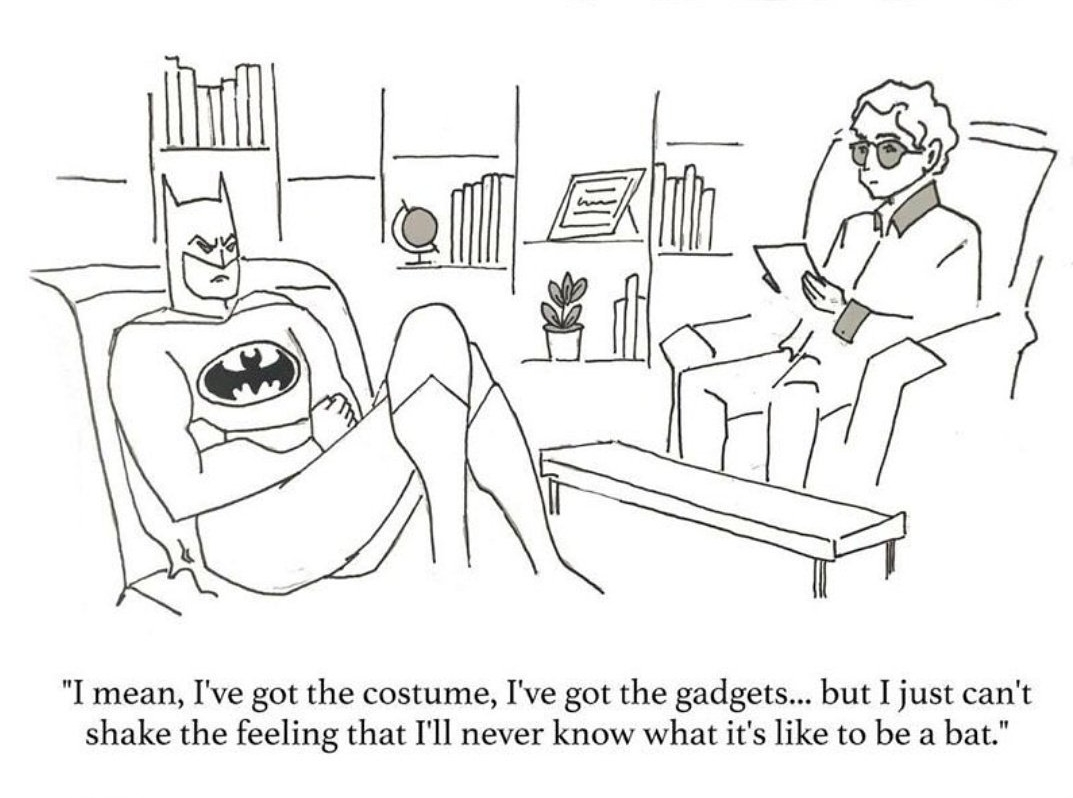
\includegraphics[width=0.7\textwidth]{to-be-a-bat}
    \caption {Is there something that it is like to be a particular, conscious thing?}
  \end{figure}
\end{frame}

\begin{frame}{Zombies, Kirk 2006}
  \begin{figure}
    \centering
    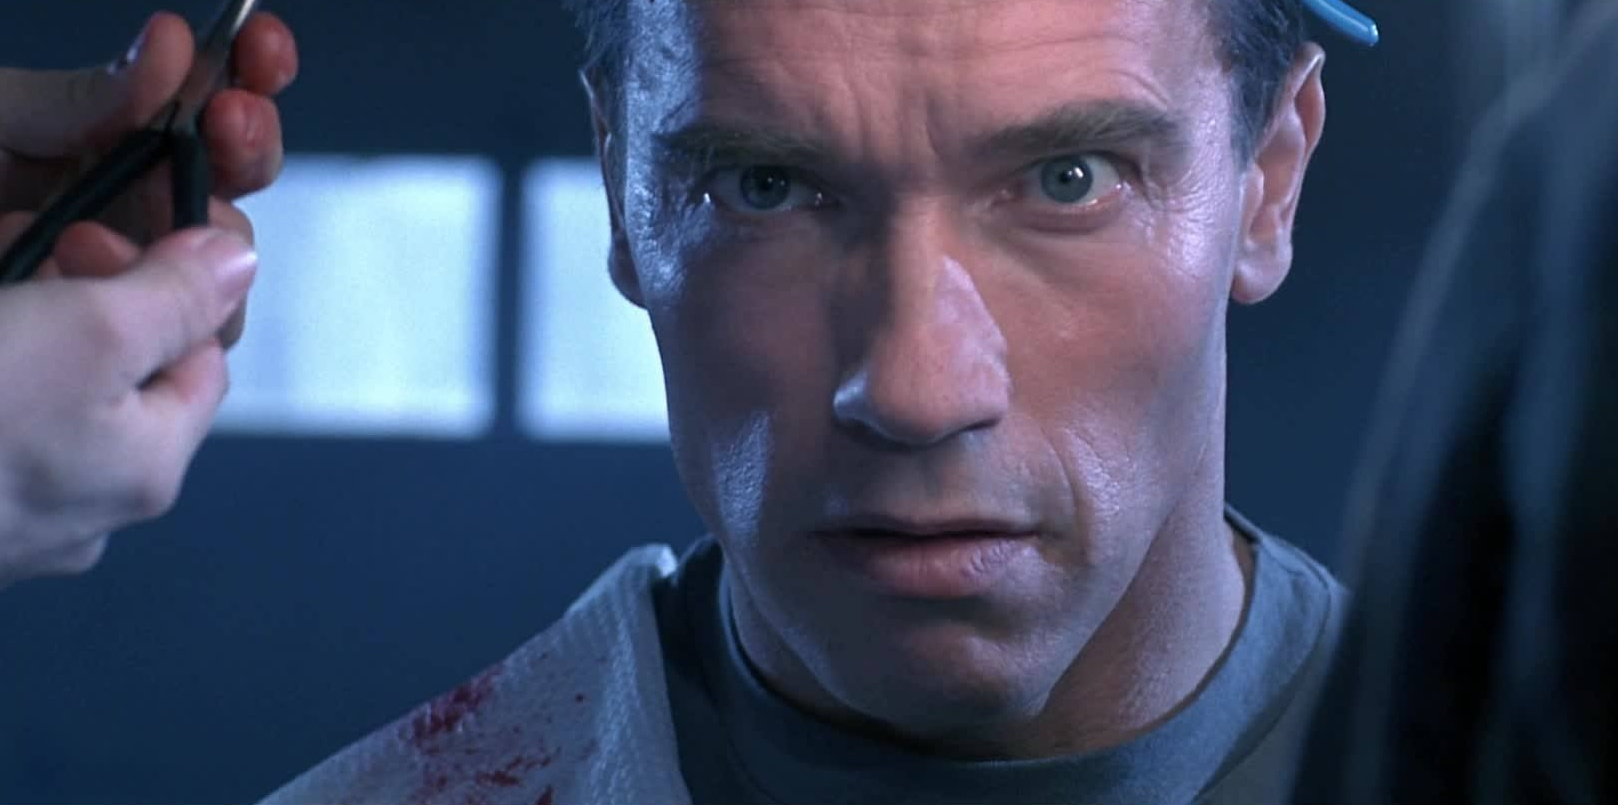
\includegraphics[width=0.9\textwidth]{terminator-no-chip}
    \caption {``Ouch!'', \; but \emph{feels} no pain}
  \end{figure}
\end{frame}


\section{Independent of both matter and contigent mind}


\begin{frame}{The abstract and the particular}
\begin{figure}
  \centering
  \begin{columns}
    \column{0.5\textwidth}
    \centering
    \caption {\emph{That which is triangular}}
    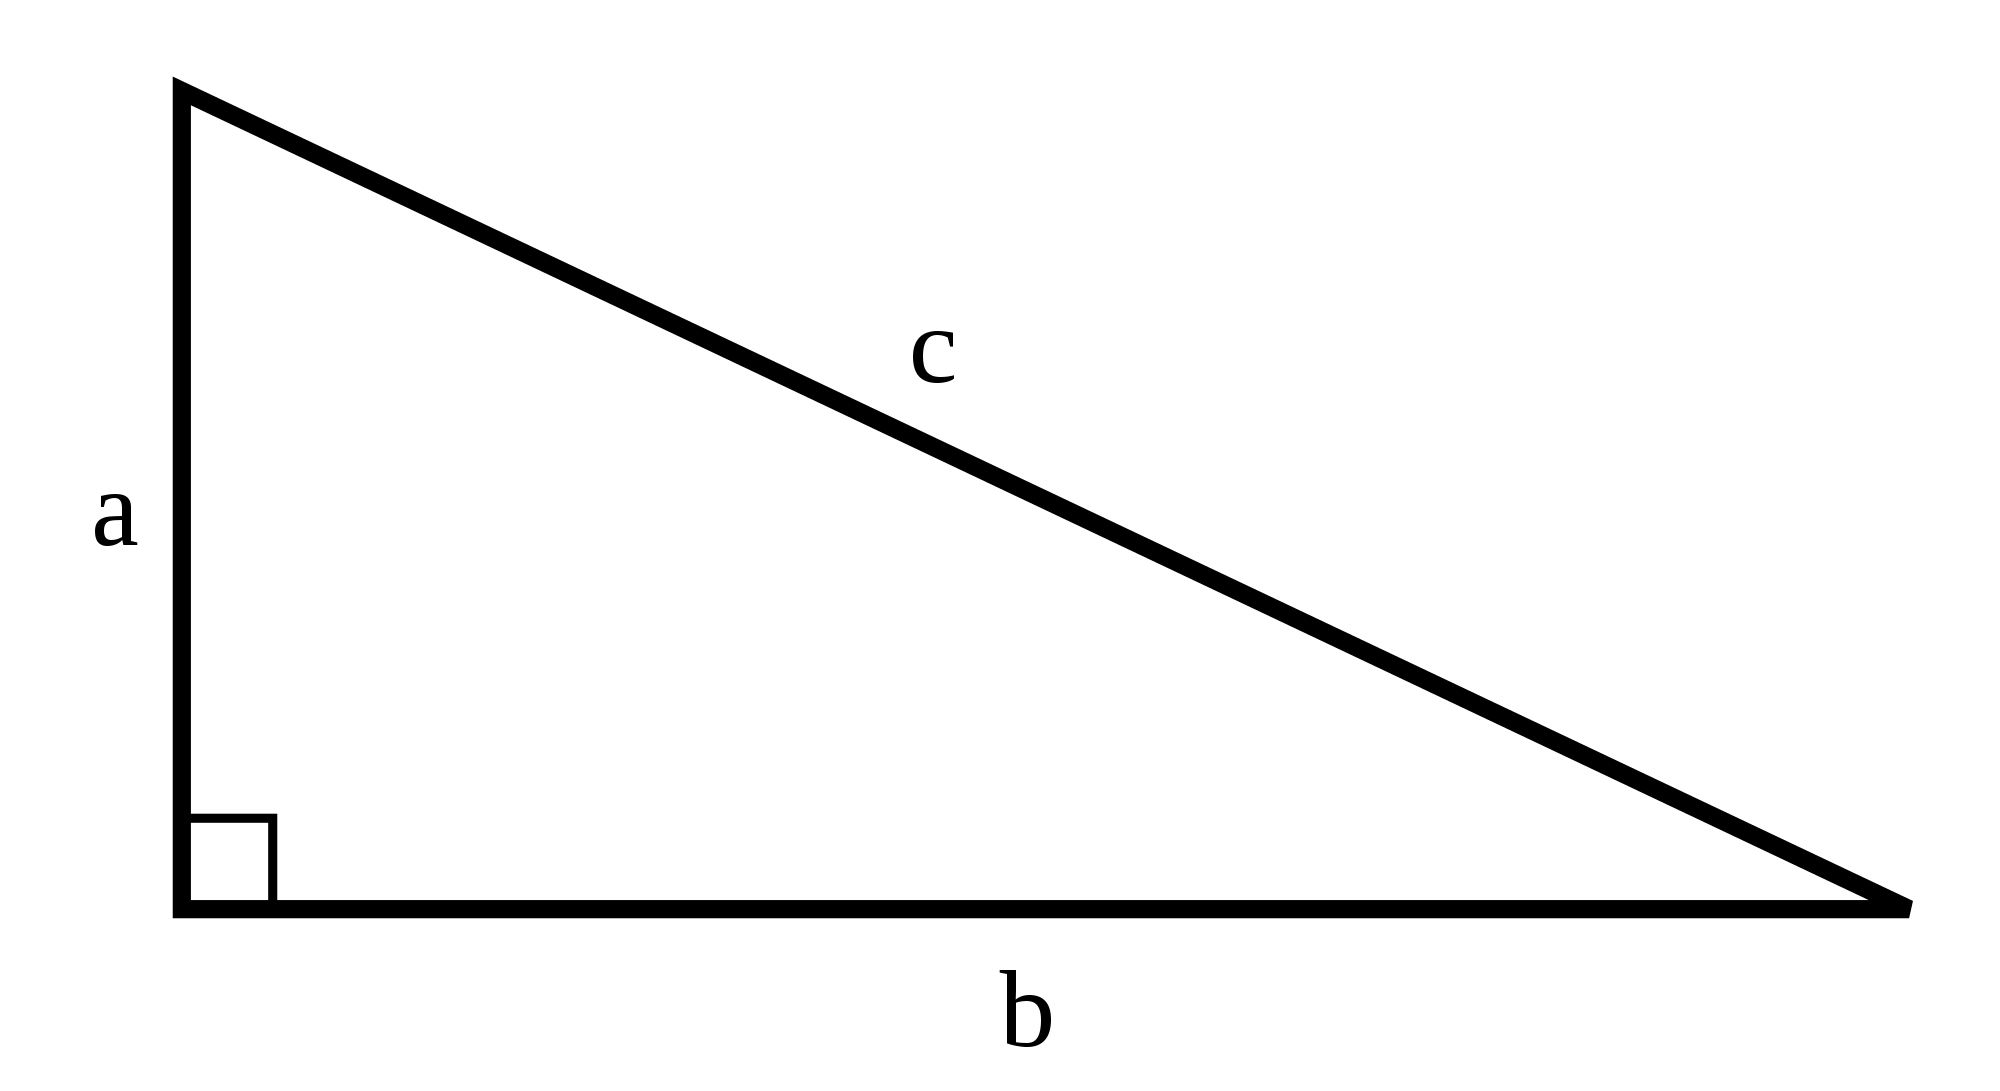
\includegraphics[width=0.99\textwidth]{triangular}
    \column{0.5\textwidth}
    \centering
    \caption {An imperfect instance}
    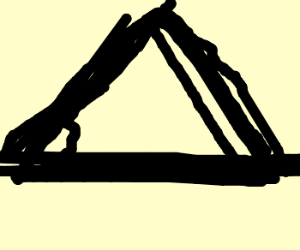
\includegraphics[width=0.99\textwidth]{triangle}
  \end{columns}
\end{figure}
I recognise something to be triangular, despite its imperfections
\end{frame}


\begin{frame}{614-609mn monochromatic light}
\begin{figure}
  \centering
  \begin{columns}
    \column{0.5\textwidth}
    \centering
    \caption {A red thing}
    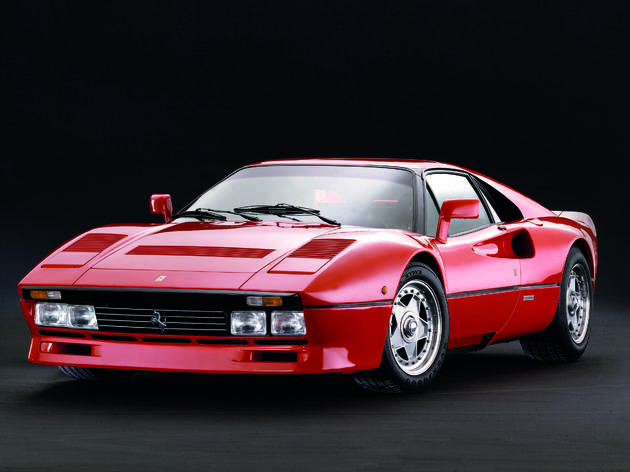
\includegraphics[width=0.99\textwidth]{ferrari}
    \column{0.5\textwidth}
    \centering
    \caption {A no entry sign with a red background}
    
\includegraphics[width=0.99\textwidth]{red_sign}
  \end{columns}
\end{figure}
Not singular in spectrum, but still conceptually singular
\end{frame}


\begin{frame}{Distant cousins}
\begin{figure}
  \centering
  \begin{columns}
    \column{0.5\textwidth}
    \centering
    \caption {Nonrational}
    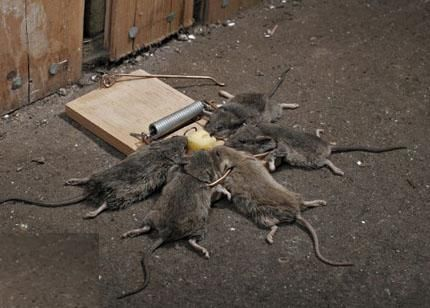
\includegraphics[width=0.99\textwidth]{mouse}
    \column{0.5\textwidth}
    \centering
    \caption {Irrational}
    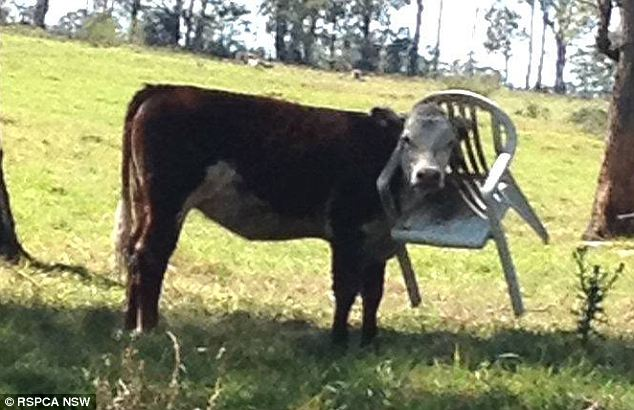
\includegraphics[width=0.99\textwidth]{cow}
  \end{columns}
\end{figure}
An individual animal is either rational or nonrational, but \emph{animality} entails neither
\end{frame}


\begin{frame}{It couldn't be otherwise}
\begin{figure}
  \centering
  \begin{columns}
    \column{0.99\textwidth}
    \centering
    \caption {It is \emph{this concept} which is commonly known}
    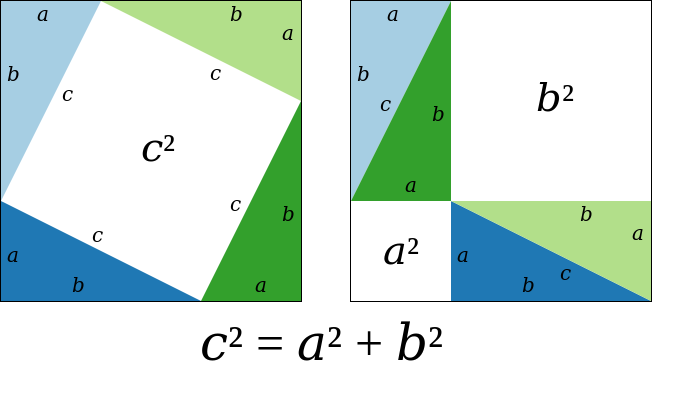
\includegraphics[width=0.8\textwidth]{pythagoras_proof}
  \end{columns}
\end{figure}
True prior to Pythagoras, and prior to matter
\end{frame}


%% Veritas est adaequatio rei et intellectus


\begin{frame}[plain]
\begin{quote}
\centering
{\Large\textbf{Veritas} est adaequatio rei et intellectus}
\end{quote}
\end{frame}


\begin{frame}{Are we talking about the same thing?}
\begin{figure}
  \centering
  \begin{columns}
    \column{0.99\textwidth}
    \centering
    \caption {``You're words are mere \emph{flatus vocis!}''}
    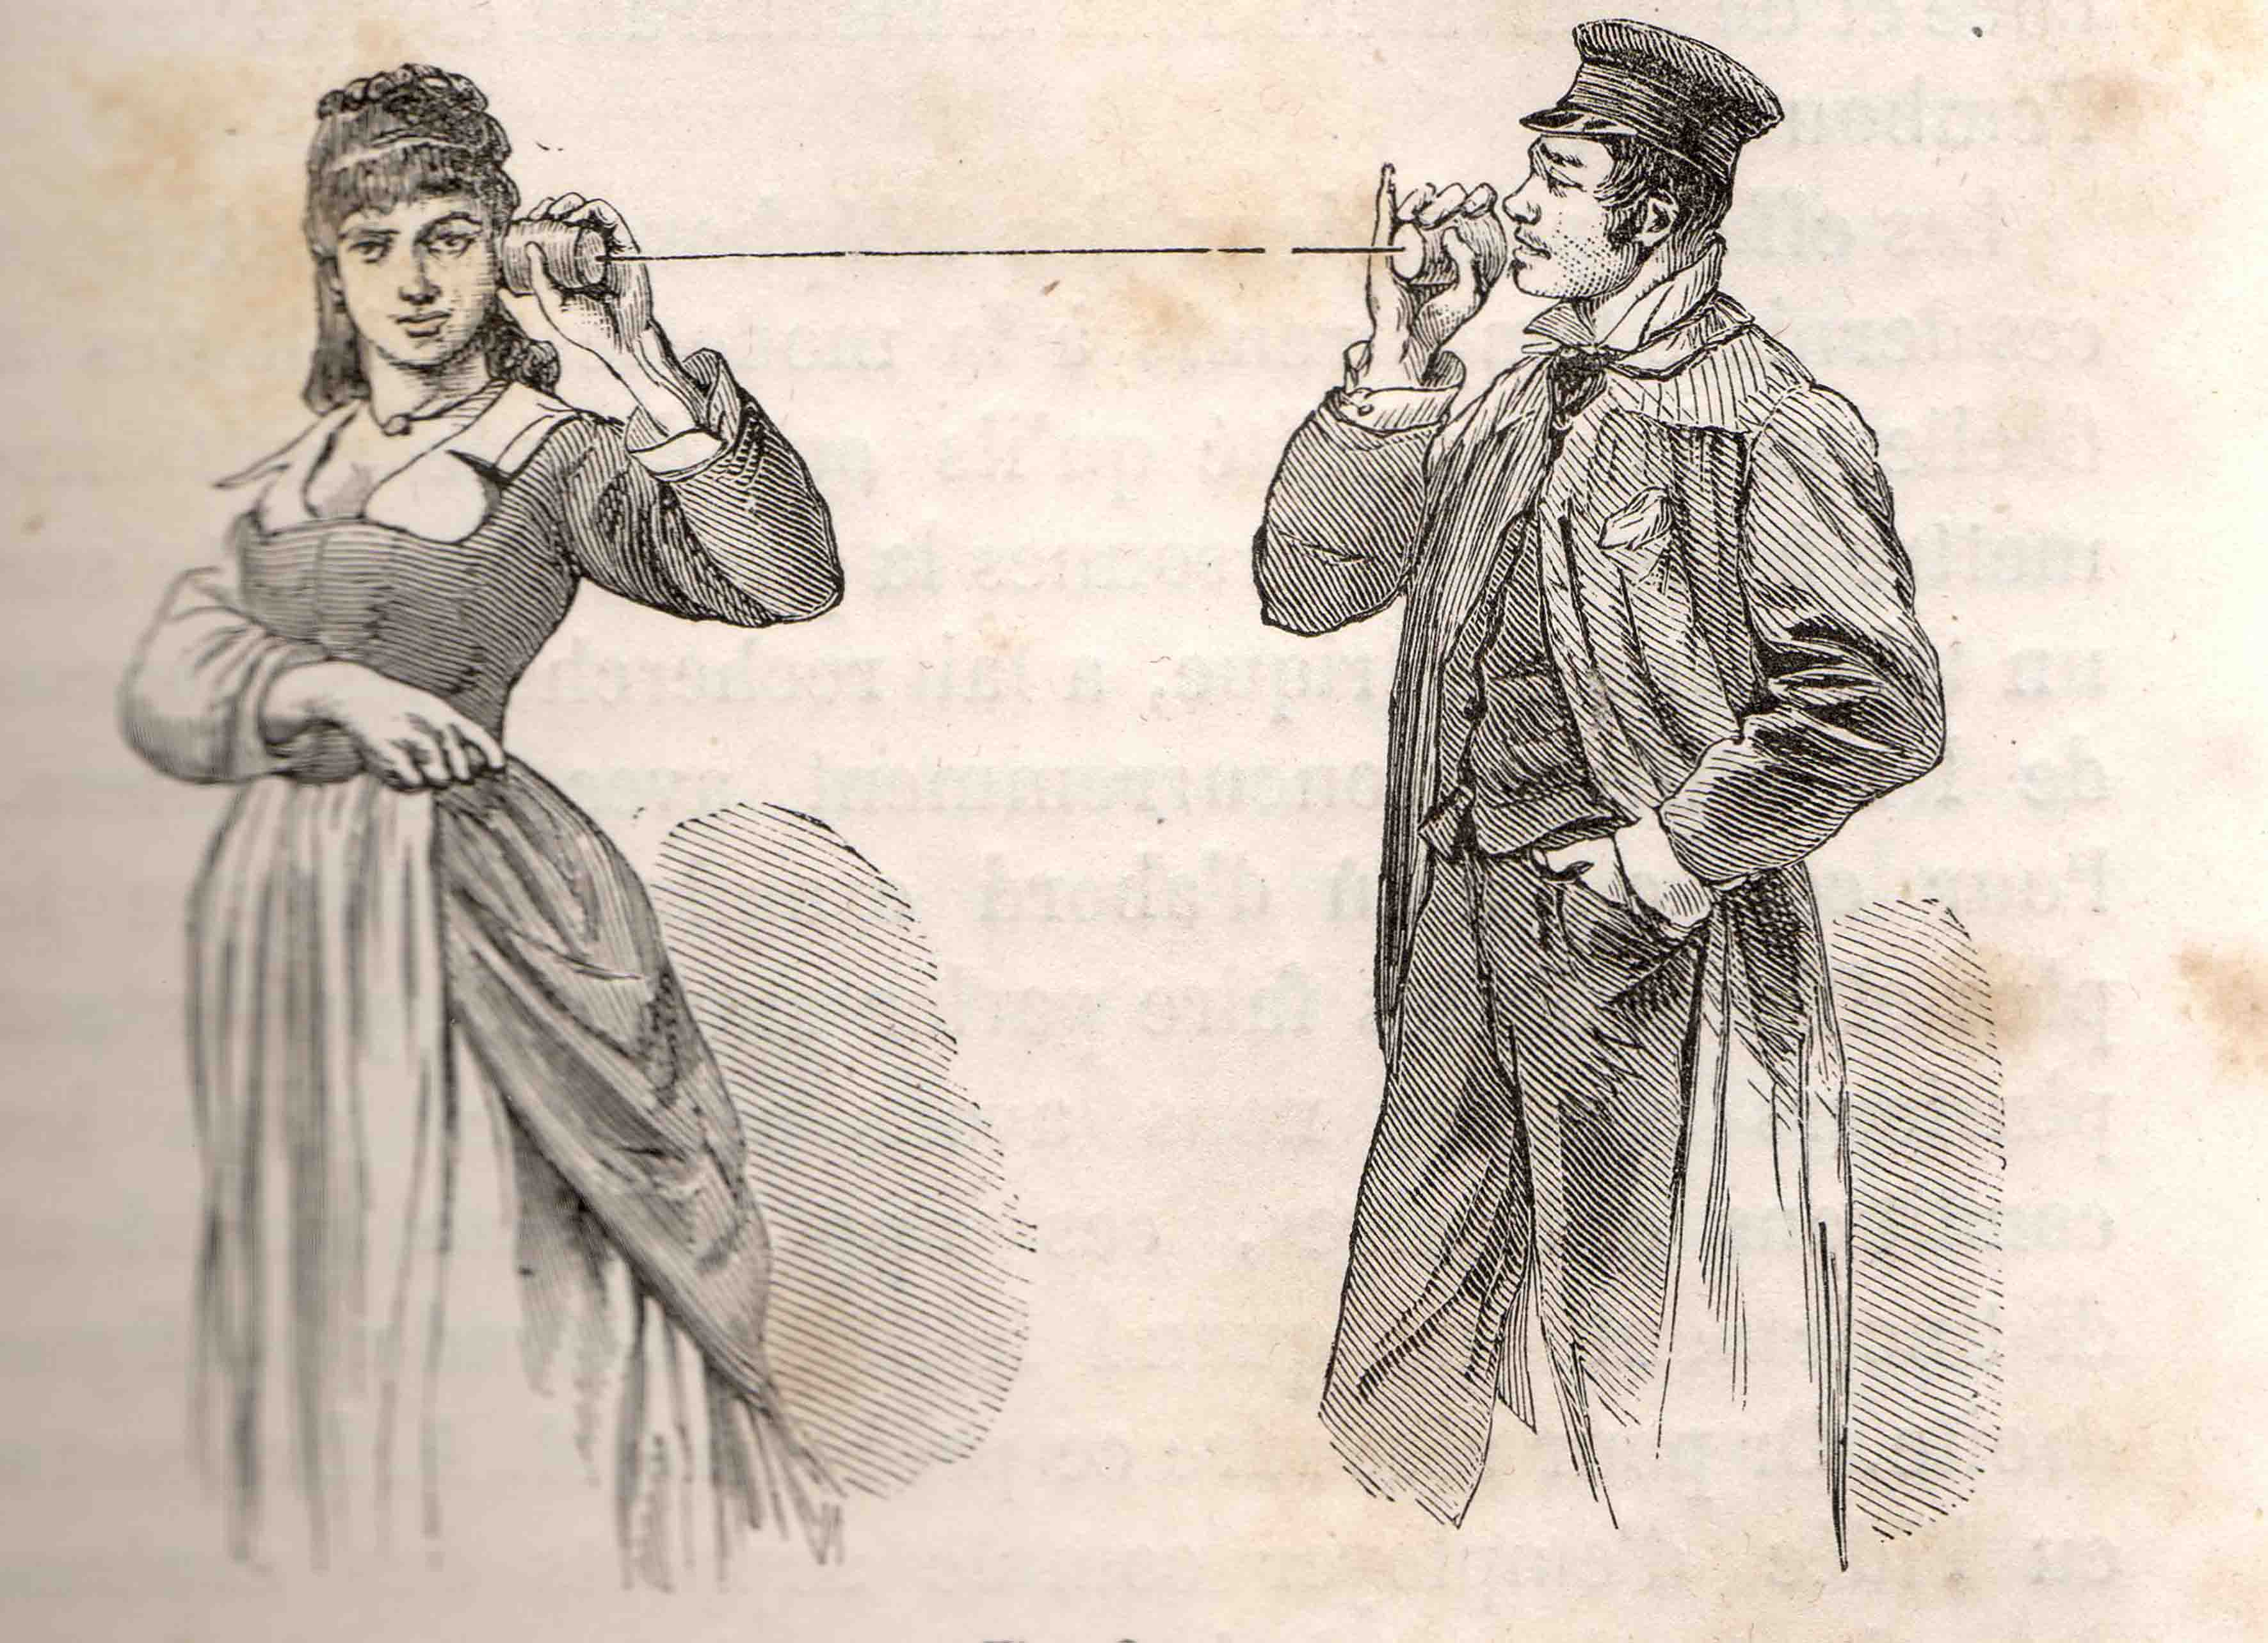
\includegraphics[width=0.6\textwidth]{communication}
  \end{columns}
\end{figure}
If we are, where is that \emph{same thing}?
\end{frame}


\section{Platonic Realism}


\begin{frame}{The Road to Reality, Penrose 2004}
  \begin{figure}
    \centering
    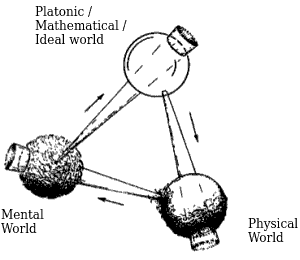
\includegraphics[width=0.55\textwidth]{three-worlds-penrose}
    \caption {\textbf{Clockwise}: mysteries,\;\; \textbf{Counter-clockwise}: prejudices}
  \end{figure}
  \centering
  \emph{adaequatio rei ad intellectum}
\end{frame}

\begin{frame}{The Road to Reality, Penrose 2004}
\textbf{Clockwise}\newline
Part of the ideal is relevant to the physical\newline
Part of the physical induces the mental\newline
Part of the mental is concerned with the ideal\newline

\textbf{Counter-clockwise}\newline
Possibility of mathematical truths inaccessible to reason\newline
Possibility of mentality not rooted in physical structures\newline
Possibility of physical action beyond the scope of mathematical control\newline
\end{frame}


\begin{frame}{The Road to Reality, Penrose 2004}
\textbf{Mysteries of the Third Realm}\newline\vspace{3mm}

Why do mathematical laws apply to the physical world with such precision?\newline\vspace{3mm}

How can some physical materials like human brains conjure up consciousness?\newline\vspace{3mm}

How is it that we can perceive mathematical truth?\newline\vspace{3mm}
\end{frame}


\section{Aristotelian Realism}


\begin{frame}{Act of abstraction to produce concepts}
  \begin{figure}
    \centering
    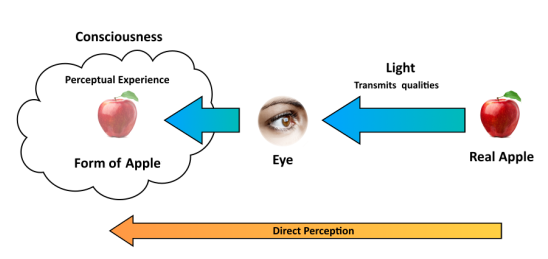
\includegraphics[width=0.9\textwidth]{aristotelian-realism}
    \caption {\emph{adaequatio intellectus ad rem}}
  \end{figure}
\end{frame}


\section{Scholastic Realism}


\begin{frame}{Act of Being}
  \begin{figure}
    \centering
    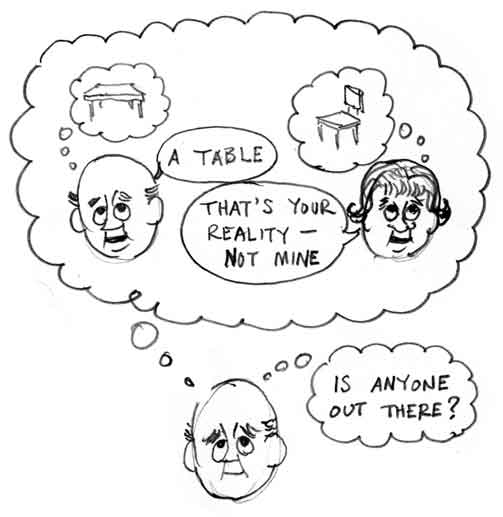
\includegraphics[width=0.5\textwidth]{scholastic-realism}
  \end{figure}
\emph{adaequatio rei ad intellectum}: Things are by participation of being
\emph{adaequatio intellectus ad rem}: I have perfectable knowledge of things
\end{frame}


\section{Nominalism}


\begin{frame}{Just a particular act, nothing more}
  \begin{figure}
    \centering
    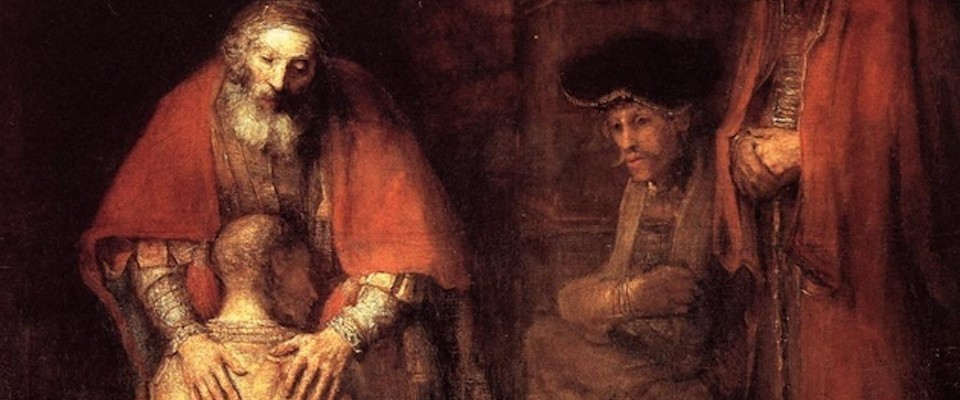
\includegraphics[width=0.9\textwidth]{mercy-rembrandt}
  \end{figure}
  \emph{Why should mercy be shown him?} \vspace{2mm}

\indent \; \; Well, it wouldn't be mercy otherwise
\end{frame}


\section{Conceptualism}


\begin{frame}{``Because I say it's art''}
  \begin{figure}
    \centering
    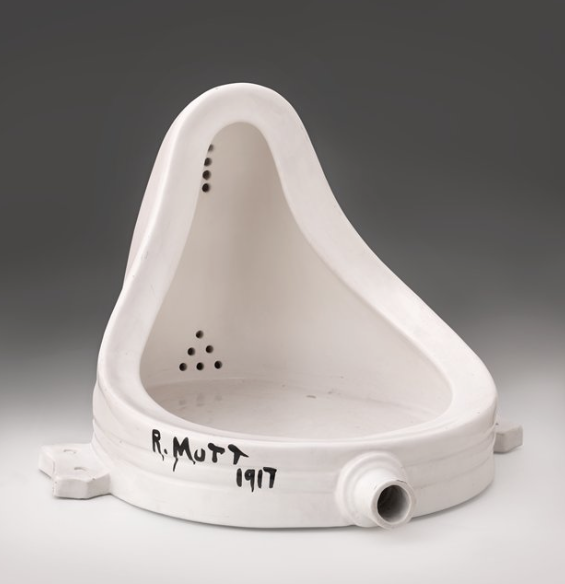
\includegraphics[width=0.6\textwidth]{toilet-duchamp}
    \caption {\emph{Fountain}, Duchamp 1917}
  \end{figure}
\end{frame}


\section{Footnotes}


\begin{frame}{Act of the intellect}
\textbf{Simple Apprehension}\newline
Intention: \emph{Essences or Natures}\newline
Product: \emph{Concept}\newline
Characteristics: \emph{Clear or Unclear}\newline
Question: \emph{What?}\newline

\textbf{Judgement}\newline
Intention: \emph{Acts of Existence}\newline
Product: \emph{Proposition}\newline
Characteristic: \emph{True or False}\newline
Question: \emph{Whether?}\newline

\textbf{Reasoning}\newline
Intention: \emph{Causes or Reasons}\newline
Product: \emph{Argument}\newline
Characteristics: \emph{Valid or Invalid}\newline
Question: \emph{Why?}\newline
\end{frame}


\end{document}
